\chapter{Association Analysis}

\textbf{Association Rule Mining} refers to, given a set of transactions, finding rules that will predict the occurrence of an item based on the occurrences of other items in the transaction

\section{Basic Concepts}

\subsection{Frequent Itemset}
An \textbf{itemset} is a collection of one or more items. An itemset with $k$ items is called a $k$-itemset.

An itemset is \textbf{frequent} if its \textbf{support} (the fraction of transactions that contain the itemset) is greater than or equal to a user-specified minimum support threshold.

\begin{table}[htbp]
   \centering
   \begin{tabular}{|c|c|}
      \hline
      Transaction ID & Items Purchased \\
      \hline
      1              & Bread, Milk         \\
      2              & Bread, Diaper, Beer, Eggs            \\
      3              & Milk, Coke, Beer, Diaper            \\
      4              & Bread, Milk, Beer, Diaper         \\
      5              & Bread, Milk, Diaper, Coke            \\
      \hline
   \end{tabular}
   \caption{Example of transactions}
   \label{tab:itemset}
\end{table}

\begin{itemize}
   \item Itemset - ${Milk,Bread,Diaper}$
   \item Suppport count ($\sigma$) - Frequency of occurrence of an itemset - $\sigma({Milk,Bread,Diaper}) = 2$
   \item Support - Fraction of transactions that contain an itemset - $s({Milk,Bread,Diaper})=\frac{2}{5}$
   \item An itemset whose support is greater than or equal to a \textit{minsup} threshold is called a frequent itemset.
   \item Association Rule - An implication expression of the form $X \Rightarrow Y$, where $X$ and $Y$ are itemsets - ${Milk,Diaper} \Rightarrow {Beer}$
   \item Rule Evaluation Metrics - 
   \begin{itemize}
      \item Support ($s$) - The proportion of transactions that contain the itemset .
      \item Confidence ($c$) - The proportion of the transactions that contain $X$ which also contain $Y$.
   \end{itemize}
\end{itemize}

Given a set of transactions T, the goal of association rule mining is to find all rules having
\begin{itemize}
	\item support $\geq$ \textit{minsup} threshold
	\item confidence $\geq$ \textit{minconf} threshold
\end{itemize}
\note{
Brute-force approach:
\begin{itemize}
	\item List all possible association rules
	\item Compute the support and confidence for each rule
	\item Prune rules that fail the minsup and minconf
thresholds
\end{itemize}

\ul{Computationally prohibitive!}}

Two-step approach:
\begin{itemize}
	\item Frequent Itemset Generation - Generate all itemsets whose support $\geq$ \textit{minsup}
   \note{This is still computationally expensive}
	\item Rule Generation - Generate high confidence rules from each frequent itemset, where each rule is a binary partitioning of a frequent itemset
\end{itemize}

% // TODO get done with 17_association_analysis_2023 

\section{Apriori Algorithm}
The purpose of the Apriori algorithm is to find all frequent itemsets in a transaction database, which means \ul{identifying itemsets that satisfy the support constraint} (threshold), i.e. finding all itemsets whose support is greater than or equal to a user-specified minimum support threshold.

The Apriori principle holds due to the following property of support of the support measure:
\begin{definition}
   [Anti-monotone Property]
   Anti-monotone property of support is formulated as:
   \[
      \forall X,Y : (X \subseteq Y) \Rightarrow s(X) \geq s(Y)
   \]
   This states that the \ul{support of an itemset never exceeds the support of its
   subsets}.
\end{definition}

\begin{algorithm}[H]
\caption{Apriori Algorithm}
\begin{algorithmic}[1]
\State $k \gets 1$
\State $F_1 \gets \{\text{frequent 1-itemsets}\}$ \Comment{Scan database and count support of each item}
\Repeat
\State $L_{k+1} \gets$ \textbf{Candidate Generation} from $F_k$ \Comment{Generate candidate $(k+1)$-itemsets}
\State $L_{k+1} \gets$ \textbf{Candidate Pruning} of $L_{k+1}$ \Comment{Prune candidates with infrequent $k$-subsets}
\State Scan transaction database to count support of each candidate in $L_{k+1}$
\State $F_{k+1} \gets$ candidates in $L_{k+1}$ with support $\geq$ minsup
\State $k \gets k + 1$
\Until{$F_k = \emptyset$}
\State \Return $\bigcup_k F_k$ \Comment{Return all frequent itemsets}
\end{algorithmic}
\end{algorithm}

% \begin{algorithm}
%    [Apriori Algorithm]
%    \begin{enumerate}
%       \item Initialize $k=1$. 
%       \item Find all $F_1 = \{\textit{frequent 1-itemsets}\}$ by scanning the transaction database and counting the support of each item.
%       \item Repeat until no new frequent itemsets are found (i.e. $F_k = \emptyset$):
%       \begin{enumerate}
%          \item \textbf{Candidate Generation} - Generate candidate $L_{k+1} = (k+1)$-itemsets from the set $F_k$ of frequent $k$-itemsets found in the previous iteration.
%          \item \textbf{Candidate Pruning} - Prune candidate itemsets in $L_{k+1}$ that have any subset (of size $k$) that are infrequent (not in $F_k$).
%          \item \textbf{Support Counting} - Scan the transaction database to count the support of each candidate in $L_{k+1}$.
%          \item \textbf{Candidate Elimination} - Eliminate candidates in $L_{k+1}$ that do not satisfy the minimum support threshold to form the set of frequent $(k+1)$-itemsets $F_{k+1}$, leaving only those candidates that are frequent.
%          \item  - Increment $k$ by 1.
%       \end{enumerate}
%    \end{enumerate}
% \end{algorithm}

\begin{definition}
   [Closed Itemset]
   An itemset X is \textbf{closed} if none of its immediate supersets
   has the same support as the itemset X.\\
   X is not closed if at least one of its immediate supersets
   has support count as X.
\end{definition}

\begin{paracol}{2}
   \colfill
\begin{table}[H]
   \centering
   \begin{tabular}{|c|c|}
      \hline
      TID & Items \\
      \hline
      1   & \{A, B\}         \\
      2   & \{B, C, D\}            \\
      3   & \{A, B, C, D\}            \\
      4   & \{A, B, D\}         \\
      5   & \{A, B, C, D\}            \\
      \hline
   \end{tabular}
   \caption{Example Transaction Database}
   \label{tab:08/exampleTransactionDB}
\end{table}
   \colfill

\switchcolumn

\begin{table}[H]
   \centering
   \begin{tabular}{|c|c|}
      \hline
      Itemset & Support \\
      \hline
      \{A\} & 4 \\
      \{B\} & 5 \\
      \{C\} & 3 \\
      \{D\} & 4 \\
      \{A,B\} & 4 \\
      \{A,C\} & 2 \\
      \{A,D\} & 3 \\
      \{B,C\} & 3 \\
      \{B,D\} & 4 \\
      \{C,D\} & 3 \\
      \{A,B,C\} & 2 \\
      \{A,B,D\} & 3 \\
      \{A,C,D\} & 2 \\
      \{B,C,D\} & 2 \\
      \{A,B,C,D\} & 2 \\
      \hline
   \end{tabular}
   \caption{Frequent Itemsets and Their Support}
   \label{tab:08/frequent_itemsets}
\end{table}
\end{paracol}

\subsection{Closed Itemsets}

From the example above, the \textbf{closed itemsets} are:
\begin{itemize}
   \item \{B\} with support 5 - closed because its immediate superset \{A,B\} has support 4 $\neq$ 5
   \item \{A,B\} with support 4 - closed because its immediate supersets \{A,B,C\} and \{A,B,D\} have support 2 and 3 respectively, both $\neq$ 4
   \item \{B,D\} with support 4 - closed because its immediate superset \{A,B,D\} has support 3 $\neq$ 4 and \{B,C,D\} has support 2 $\neq$ 4
   \item \{A,B,D\} with support 3 - closed because its immediate superset \{A,B,C,D\} has support 2 $\neq$ 3
   \item \{C,D\} with support 3 - closed because its immediate supersets have different support
   \item \{A,B,C,D\} with support 2 - closed because it has no supersets
\end{itemize}

Examples of \textbf{non-closed itemsets}:
\begin{itemize}
   \item \{A\} with support 4 is \textbf{not closed} because its immediate superset \{A,B\} has the same support 4
   \item \{A,C\} with support 2 is \textbf{not closed} because its immediate superset \{A,B,C\} has the same support 2
   \item \{A,B,C\} with support 2 is \textbf{not closed} because its immediate superset \{A,B,C,D\} has the same support 2
\end{itemize}

Closed itemsets are important because they provide a compact representation of all frequent itemsets while preserving complete support information.

\subsection{Maximal Itemsets}

\begin{definition}
   [Maximal Itemset]
   An itemset X is \textbf{maximal} if none of its immediate supersets
   is frequent.\\
   X is not maximal if at least one of its immediate supersets
   is frequent.
\end{definition}

Assuming a minimum support threshold of 2, the \textbf{maximal frequent itemsets} from the example are:
\begin{itemize}
   \item \{B\} with support 5 - maximal if we consider only singleton itemsets, but \textbf{not maximal} overall because its supersets \{A,B\}, \{B,C\}, \{B,D\} are frequent
   \item \{A,B,D\} with support 3 - maximal because its only superset \{A,B,C,D\} has support 2, which is still frequent, so \textbf{not maximal}
   \item \{B,D\} with support 4 - \textbf{not maximal} because its superset \{A,B,D\} is frequent
   \item \{C,D\} with support 3 - \textbf{not maximal} because its supersets \{A,C,D\}, \{B,C,D\}, and \{A,B,C,D\} are frequent (support $\geq$ 2)
   \item \{A,B,C,D\} with support 2 - \textbf{maximal} because it has no supersets and it is frequent
\end{itemize}

Therefore, with minsup = 2, the only \textbf{maximal frequent itemset} is:
\begin{itemize}
   \item \{A,B,C,D\} with support 2
\end{itemize}

\note{
   Every maximal frequent itemset is also closed, but not every closed itemset is maximal. Maximal itemsets provide an even more compact representation than closed itemsets, but they only preserve information about which itemsets are frequent, not their exact support counts.
}

\begin{figure}[htbp]
   \centering
   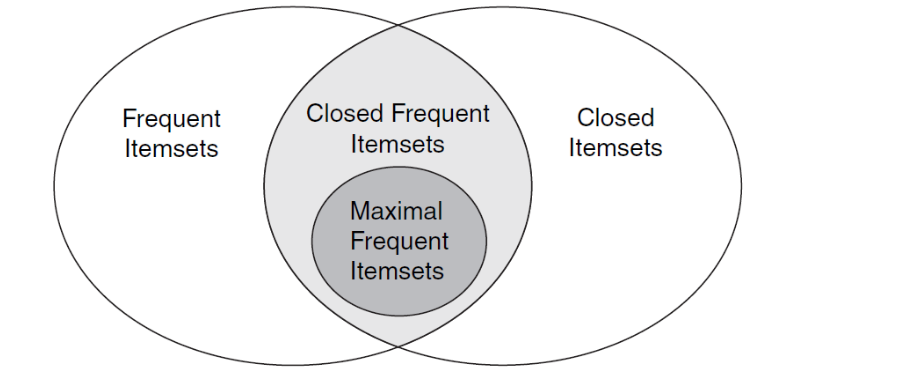
\includegraphics{images/08/sets.png}
   \caption{Relationships between frequent, closed, closed frequent and maximal frequent itemsets}
   \label{fig:08/sets}
\end{figure}

\section{Confidence}
The \textbf{confidence} of an association rule $X \Rightarrow Y$ is a measure of the reliability of the rule. It is defined as the conditional probability that a transaction contains the itemset $Y$ given that it contains the itemset $X$. Mathematically, confidence is expressed as:
\[c(X \Rightarrow Y) = \frac{s(X \cup Y)}{s(X)}\]
where:
\begin{itemize}
   \item $s(X \cup Y)$ is the support of the itemset that contains both $X$ and $Y$.
   \item $s(X)$ is the support of the itemset $X$.
\end{itemize}

The confidence value ranges from 0 to 1, where a higher confidence indicates a stronger association between the itemsets $X$ and $Y$. For example, a confidence of 0.8 means that 80\% of the transactions that contain $X$ also contain $Y$.

\subsection{Drawbacks}

Confidence has some drawbacks:
\begin{itemize}
   \item It does not consider the overall frequency of the consequent itemset $Y$ in the dataset.
   \item It can be misleading in cases where the consequent itemset $Y$ is very common in the dataset, leading to high confidence values even when there is no real association between $X$ and $Y$.
\end{itemize}
\note{To address these issues, other measures such as \textbf{lift} and \textbf{conviction} are often used in conjunction with confidence to provide a more comprehensive evaluation of association rules.}

\subsubsection{What rules do we want}
\begin{itemize}
	\item Confidence$(X \Rightarrow Y)$ should be sufficiently high
	\begin{itemize}
		\item To ensure that people who buy $X$ will more likely buy $Y$ than not buy $Y$
	\end{itemize}
	\item Confidence$(X \Rightarrow Y) > support(Y)$
	\begin{itemize}
		\item Otherwise, rule will be misleading because having item $X$ actually reduces the chance of having item $Y$ in the same transaction
	\end{itemize}
	\item Is there any measure that capture this constraint?
	\begin{itemize}
		\item Answer: \textit{Yes}. There are many of them.
	\end{itemize}
\end{itemize}

\section{Other criteria}
$ \textit{confidence}(X \Rightarrow Y) = support(Y)$ is equivalent to:
\begin{align*}
   P(Y|X) = P(Y)\\
   P(X,Y) = P(X)P(Y) \qquad \text{(independence)}
\end{align*}

\begin{align*}
   P(X,Y) < P(X)P(Y) \qquad \text{(negative correlation)}\\
   P(X,Y) > P(X)P(Y) \qquad \text{(positive correlation)}
\end{align*}


\subsection{Lift}
The \textbf{lift} of an association rule $X \Rightarrow Y$ is a measure of how much more likely the occurrence of itemset $Y$ is when itemset $X$ is present, compared to when $Y$ occurs independently of $X$. It is defined as:
\[\text{lift}(X \Rightarrow Y) = \frac{c(X \Rightarrow Y)}{s(Y)} = \frac{s(X \cup Y)}{s(X) \times s(Y)}\]
where:
\begin{itemize}
   \item $c(X \Rightarrow Y)$ is the confidence of the rule.
   \item $s(Y)$ is the support of the itemset $Y$.
\end{itemize}

In the slides it is defined as:
\[\text{lift}(X \Rightarrow Y) = \frac{P(X,Y)}{P(X) \times P(Y)}\]

A lift value greater than 1 indicates a positive association between $X$ and $Y$, meaning that the presence of $X$ increases the likelihood of $Y$. A lift value less than 1 indicates a negative association, while a lift value equal to 1 suggests that $X$ and $Y$ are independent.
\note{Lift is particularly useful for identifying interesting rules that may not be apparent from confidence alone, as it accounts for the overall frequency of the consequent itemset $Y$ in the dataset.}

\subsection{Interest}
The \textbf{interest} of an itemset $X$ is a measure of how much the actual support of $X$ deviates from what would be expected if the items in $X$ were independent. It is defined as:
\[\text{interest}(X) = s(X) - \prod_{i \in X} s(\{i\})\]
where:
\begin{itemize}
   \item $s(X)$ is the support of the itemset $X$.
   \item $\prod_{i \in X} s(\{i\})$ is the product of the supports of the individual items in $X$.
\end{itemize}

In the slides it is defined as:
\[\text{interest}(X) = \frac{P(X,Y)}{P(X),P(Y)}\]

A positive interest value indicates that the items in $X$ co-occur more frequently than would be expected under independence, suggesting a positive association. A negative interest value indicates that the items co-occur less frequently than expected, suggesting a negative association. An interest value of zero suggests that the items are independent.

\subsection{Other measures}
In the slide two other measures are defined:
\begin{align*}
   PS = P(X,Y) - P(X)P(Y) \\
   \sigma \textit{-coefficient} = \frac{P(X,Y) - P(X)P(Y)}{\sqrt{P(X)P(Y)(1-P(X))(1-P(Y))}}
\end{align*}
These measures also aim to capture the degree of association between itemsets, taking into account their individual supports and the expected co-occurrence under independence.

\section{Non-binary Attributes}

\begin{figure}[htbp]
   \centering
   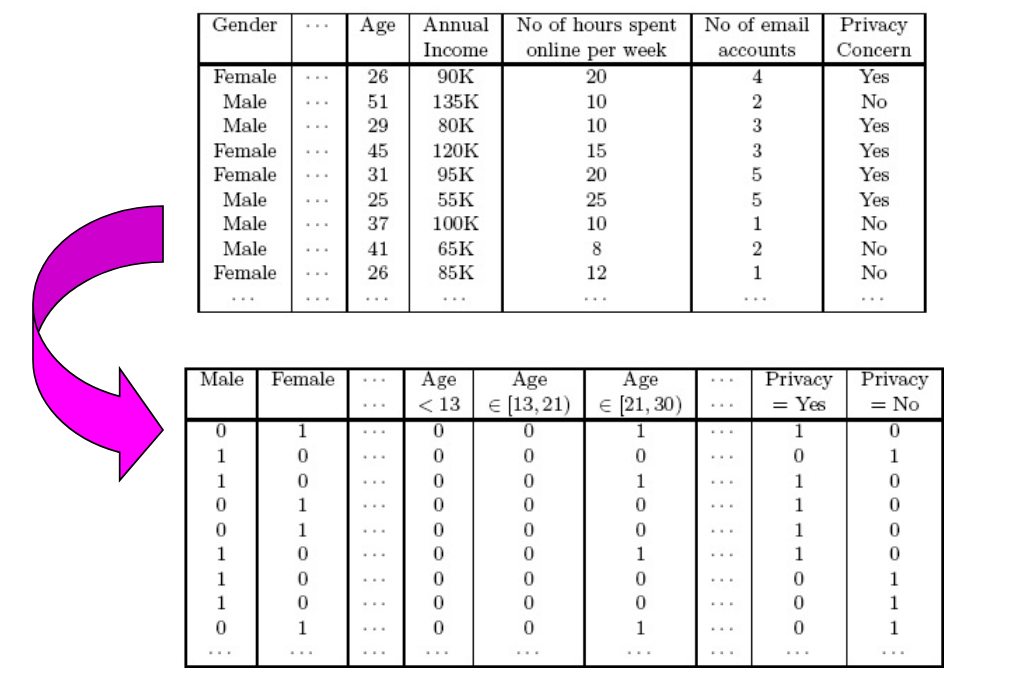
\includegraphics{images/08/nonbinary.png}
   \caption{Handling non-binary attributes by changing the actual columns}
   \label{fig:08/nonbinary}
\end{figure}

\subsection{Categorical attributes}
Categorical attributes are variables that can take on a limited, fixed number of possible values, representing distinct categories or groups. These attributes are often used in data mining and machine learning tasks to classify or group data points based on their characteristics.

We have to apply association analysis to non-asymmetric binary attributes, so we have to formulate rules like:
\[
   {Gender=Male, Age \in [21,30)} \Rightarrow {No of hours online \geq 10}
\]

Some attributes can have many possible values, with many of these values having very low support. To deal with this, we can use \textbf{attribute
generalization}, which involves replacing specific attribute values with more general categories based on a predefined \textbf{hierarchy} or \textbf{taxonomy}.
For example, instead of using specific ages, we can group them into age ranges like [0-10), [10-20), [20-30), etc. This helps to reduce the number of distinct values and increases the support for each category, making it easier to identify meaningful patterns in the data.

In some other cases we also may have a hierarchy of values for an attribute. For example, for the attribute ``Location'', we may have a hierarchy like City $\rightarrow$ State $\rightarrow$ Country. In such cases, we can use the hierarchy to generalize the attribute values and find association rules at different levels of granularity.

\subsection{Continuous attributes}
Continuous attributes are variables that can take on an infinite number of values within a given range. These attributes are often used in data mining and machine learning tasks to represent measurements or quantities that can vary continuously.

To handle such values we have various methods:
\begin{itemize}
   \item Discretization-based
   \item Statistics-based
   \item Non-discretization (such as \textsc{minApriori})
\end{itemize}

\note{
   // TODO skipped support counting with hash tree
}